\section{Resizable Arrays Latencies}

\begin{tcolorbox}
	The implementation of the geometric expansion array and HAT can be found \href{https://github.com/nngerncham/cs315_apal/tree/main/assignments/asn01/01-better-resizable-arrays}{here}.
\end{tcolorbox}

%\subsection{Methodology}

%First, a hashed array tree (HAT) and a resizable array using geometric expansion (GE) data structures are implemented using Rust's \mintinline{rust}{Vec} to act as the `primitive' array. To ensure that the \mintinline{rust}{Vec} will not have to do its own resizing, they are always initialized using \mintinline{rust}{Vec::with_capacity(_)} so they always have an initial capacity that is decided by me. Both data structures implement the methods \mintinline{rust}{push_back(e)} for appending element \mintinline{rust}{e} to the end the array, \mintinline{rust}{get(i)} for accessing the element at index \mintinline{rust}{i}, and an internal \mintinline{rust}{expand()} that is used for expanding when full. The expansion for HAT is implemented according to Sitarski's paper from 1996.

%Once both data structures are implemented, $N = 2^{20} \approx 1,000,000$ elements are appended and measured for latency. The assembly instruction \mintinline{asm}{rdtsc} is used to precisely measure the latency between the start of an append until the end. Once the elements are appended, both data structures are accessed at random indices repeatedly and measured for latency. The indices are randomized independently of each other. Once finished, both data structures are then scanned from left to right and measured for latency. Finally, to measure the overall throughput, a new instance of each data structure created and $N$ elements are then appended to them. The \textit{timer} starts before the data structure is created and stops after everything has been appended. This is repeated $M = 100$ times and recorded.

%\subsection{Results}

\begingroup

\subsection{Append Latency}

\begin{figure}[H]
	\begin{center}
		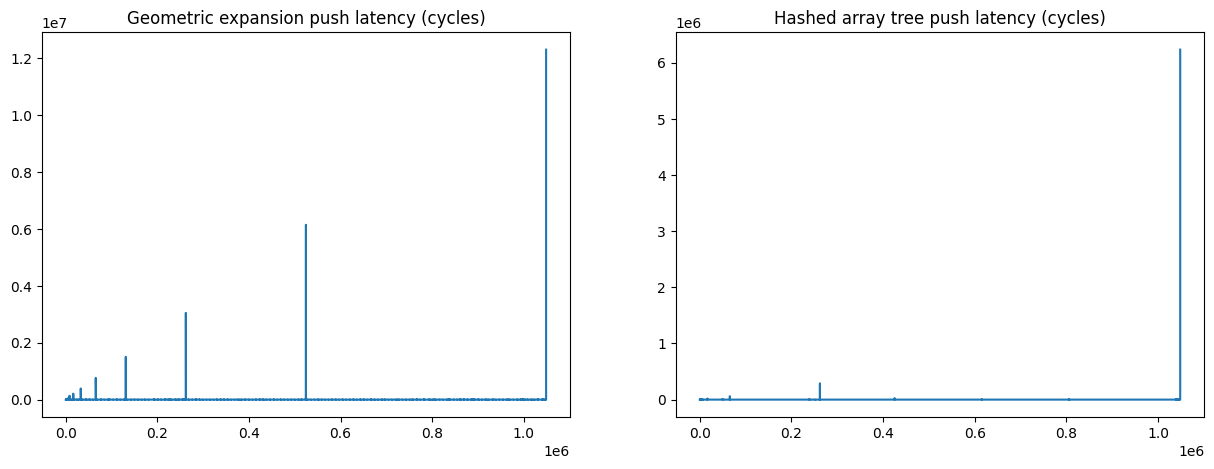
\includegraphics[width=0.9\textwidth]{01-push-latencies.png}
		\caption{Push latencies of different implementations of resizable arrays}
		\label{fig:push-latency}
	\end{center}
\end{figure}

From the axes themselves, it seems like HATs take significantly longer for each of its expansion, especially the later ones since copying elements from one HAT to another is significantly more complicated than copying one array to another in the implementation with geometric expansion (GE). However, the frequency of HATs expanding is significantly lower than with GE as there aren't as many latency spikes in the HAT compared to the GE as it clearly has more latency spikes than HATs.

\endgroup

\begingroup

\subsection{Access Latency}

\begin{figure}[H]
	\begin{center}
		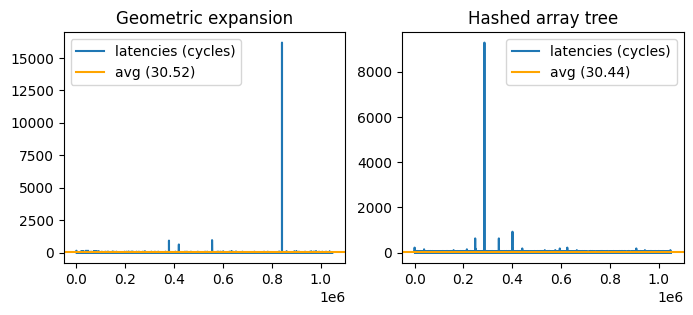
\includegraphics[width=0.9\textwidth]{01-get-latencies.png}
		\caption{Random access latencies of different implementations of resizable arrays}
		\label{fig:get-latency}
	\end{center}
\end{figure}

From the figure, there seems to be no clear difference in the pattern of access latency spikes as they seem to show up at some arbitrary point. The average latency for both data structures are also about the same at approximately 30.5 cycles. However, the highest latency for GE is higher than HAT's.

\endgroup

\begingroup

\subsection{Scan Throughput}

\begin{figure}[H]
	\begin{center}
		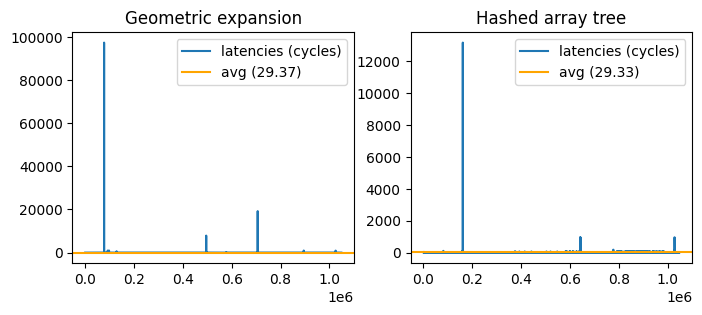
\includegraphics[width=0.9\textwidth]{01-scan-latencies.png}
		\caption{Scan latencies of different implementations of resizable arrays}
		\label{fig:scan-throughput}
	\end{center}
\end{figure}

Similar to random access latencies, scanning through both data structures seems to have no difference in average latency of about 29.35 cycles but the highest latency of GE is higher than HAT's.

\endgroup

\begingroup

\subsection{Overall Throughput}

\begin{figure}[H]
	\begin{center}
		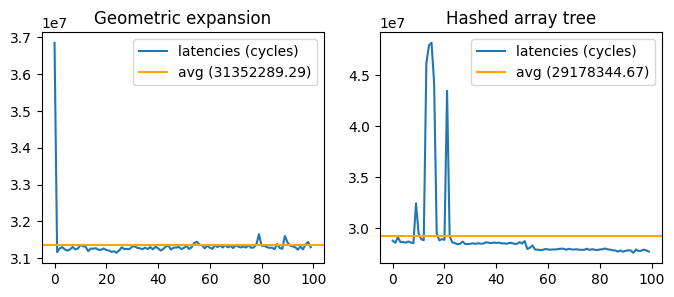
\includegraphics[width=0.9\textwidth]{01-overall-latencies.png}
		\caption{Overall throughput of different implementations of resizable arrays}
		\label{fig:overall-throughput}
	\end{center}
\end{figure}

Here is another place where we see a clear difference in cycle spike patterns. Using GE, there is only a huge spike at the beginning but the rest are rather stable. However, HAT's throughput is a completely difference story. It does not have as big as a spike in the beginning, but suddenly shoots up around iteration 10 of creating a new HAT and appending $N$ elements to it. However, it does seem to be come a lot more stable afterwards.

The interesting observation we can make is that the average throughput for GE is higher than HAT's despite having a more \textit{stable} latency after the big spike at the beginning. This is also despite the fact that the highest number of spikes for appending $N$ elements to the data structure is higher on the HAT.

\endgroup

\begingroup

\subsection{Conclusion and Limitations}

It is clear to see that on average, both data structures perform roughly the same. However, due to the implementation overhead of the HAT, I can see why most (if not all) programming languages are not using it. The only clear advantage the HAT has over GE is that it wastes less memory space and resizes less often but that also comes with its own problems since the data structure also has to allocate memory more often since the HAT is essentially a dynamically-allocated matrix.

I would like to point out that the fact that \mintinline{rust}{Vec} being used as the `primitive array' used for implementing both data structures is itself a resizable array, possibly leading to some performance overhead of its own. This could have made the test results less accurate.

\endgroup
